\documentclass{standalone}
\usepackage{tikz}
\usepackage{ctex,siunitx}
\setCJKmainfont{Noto Serif CJK SC}
\usepackage{tkz-euclide}
\usepackage{amsmath}
\usetikzlibrary{patterns, calc,3d}
\usetikzlibrary {decorations.pathmorphing,decorations.pathreplacing,decorations.shapes}
\tikzset{label style/.append style={font=\small}}
\begin{document}
\small
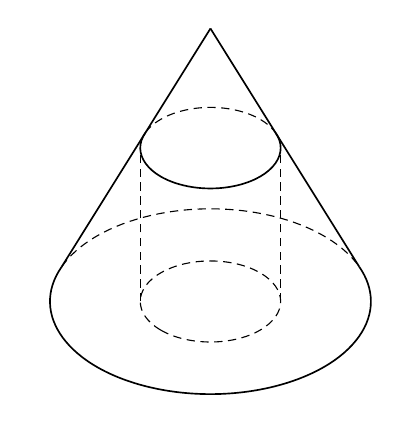
\begin{tikzpicture}[>=latex,scale=1.3,inner sep=2pt,x={(-150:8mm)},z={(-30:8mm)}]
\begin{scope}[canvas is xz plane at y=0]
  \draw[densely dashed](0,0)circle(0.7);
  \draw[semithick]({1.6*cos(-67)},{1.6*sin(-67)})arc(-67:157:1.6);
  \draw[densely dashed]({1.6*cos(-67)},{1.6*sin(-67)})arc(293:157:1.6);
\end{scope}
\begin{scope}[canvas is xz plane at y=1.5]
  \draw[semithick]({0.7*cos(-67)},{0.7*sin(-67)})arc(-67:157:0.7);
  \draw[densely dashed]({0.7*cos(-67)},{0.7*sin(-67)})arc(293:157:0.7);
\end{scope}
\draw[densely dashed]({0.7*cos(-45)},0,{0.7*sin(-45)})--({0.7*cos(-45)},1.5,{0.7*sin(-45)});
\draw[densely dashed]({0.7*cos(135)},0,{0.7*sin(135)})--({0.7*cos(135)},1.5,{0.7*sin(135)});
\draw[semithick](0,8/3,0)--({1.6*cos(-67)},0,{1.6*sin(-67)});
\draw[semithick](0,8/3,0)--({1.6*cos(157)},0,{1.6*sin(157)});
\end{tikzpicture}
\end{document}